\chapter{Real world implementation}
\label{cap:real_implementation}

\intro{In this chapter, we will discuss the implementation of the proposed solution based on a real-world scenario presented to the company by a client during the internship period. The client is a company that specializes in high-performance protective gear and technical apparel for motorsports and action sports enthusiasts. The goal of the project was to develop a system that could analyze IMU data from a rider's suit and provide feedback on the rider's performance. The client wanted to use this system to improve the rider's performance both for road users and motorsport pilots.}\\

\section{Client's requirements}
\label{sec:client_requirements}
The problem involves managing and processing data collected from various Motorcycle suits used by private and professional users. These products, used in different scenarios, generate data that needs to be efficiently collected, processed, stored, and analyzed to provide insights and ensure user safety and satisfaction. The solution must handle sporadic and intensive data uploads, support multiple types of users and devices, and ensure data integrity and accessibility.

\subsection*{User Types and Usage Patterns}
\begin{itemize}
    \item \textbf{Private Users with Sporadic Use}: Upload data approximately once a week.
    \item \textbf{Private Users with Intensive Use}: Upload data approximately three times a week.
    \item \textbf{Private Users with Multiple Products}: Use multiple products based on the scenario (e.g., road, track, off-road), with each of them offering different levels of protection. The products are classified into two categories:
    \begin{itemize}
        \item \textbf{Lightweight Protection}: Daily usage, data uploads three times a week.
        \item \textbf{Extended Protection}: Weekly usage (e.g. track or off-road during the weekend), data uploads once a week.
    \end{itemize}
    \item \textbf{Professional Users}: Managed by authorized technicians, data uploads five times a week.
\end{itemize}

\subsection*{Data Uploads and Storage}
\begin{itemize}
    \item \textbf{File Size}:
    \begin{itemize}
        \item Private users: 50 MB per upload.
        \item Professional users: 250 MB per upload.
    \end{itemize}
    \item \textbf{Data Volume}:
    \begin{itemize}
        \item Weekly: 3.5 TB.
        \item Yearly: 43 TB.
    \end{itemize}
\end{itemize}

\begin{center}
    \begin{table}[h]
        \centering
        \begin{tabular}{| p{4cm} | p{2cm} | p{2cm} | p{2cm} | p{2cm} |}
            \hline
            \textbf{} & \multicolumn{2}{c|}{\textbf{Private Users}} & \multicolumn{2}{c|}{\textbf{Professional Users}} \\
            \hline
            \textbf{} & \textbf{Sporadic Use} & \textbf{Intensive Use} & \textbf{Lightweight} & \textbf{Extended} \\
            \hline
            \textbf{Number of Users} & 30,000 & 10,000 & 1,000 & 30 \\
            \hline
            \textbf{Number of Uploads per Week} & 1 & 3 & 1 & 5 \\
            \hline
            \textbf{Number of Weeks per Year} & 16 \newline (4 months) & 8 \newline (2 months) & 8 \newline (2 months) & 36 \newline (9 months) \\
            \hline
            \textbf{Average File Size} & \multicolumn{2}{c|}{50 MB} & \multicolumn{2}{c|}{250 MB} \\
            \hline
            \textbf{Overall Data Volume per Week} & \multicolumn{2}{c|}{$\approx$1.5 TB} & $\approx$250 GB & $\approx$40 GB \\
            \hline
            \textbf{Overall Data Volume per Year} & $\approx$24 TB & $\approx$12 TB & $\approx$2 TB & $\approx$1.5 TB \\
            \hline
        \end{tabular}
        \caption{Data Volume Estimates}
        \label{table:data_volume}
    \end{table}
    
    
\end{center}

\subsection*{Data Handling and User Interaction}
\begin{itemize}
    \item \textbf{Data Transfer}:
    \begin{itemize}
        \item Ensure data transfer completion even with battery constraints or disconnections.
        \item Implement rules to ensure data transfer occurs only when the device is connected to a charger.
        \item Manage data consistency and state at the firmware level.
    \end{itemize}
    \item \textbf{Notifications}:
    \begin{itemize}
        \item Notify private users of new data insights via push notifications or a dedicated portal.
        \item Notify the R\&D team for professional users.
    \end{itemize}
    \item \textbf{Data Retention}:
    \begin{itemize}
        \item Metrics stored permanently.
        \item Raw data stored temporarily (2-4 weeks) unless a crash event is detected or for professional users.
        \item Users have a time window to download and save their raw data.
    \end{itemize}
\end{itemize}

\section{System Architecture}
\label{sec:system_architecture}
Considering the requirements and usage patterns, the system architecture must be designed to handle the sporadic and intensive data uploads from different types of users. The architecture must be scalable, fault-tolerant, and platform-agnostic to support future growth and changes in the system. Two different architectures were proposed to meet the client's requirements: an on-demand analysis architecture and a preemptive analysis architecture. Both architectures are based on the same core components described in \ref{sec:architecture}, but they differ in the way data is processed and analyzed.
It's also worth mentioning that even if only \href{https://www.arubacloud.com/}{Aruba Cloud}\footcite{site:aruba-cloud} was considered for this project, the system is designed to be platform-agnostic and can be deployed on any cloud provider.

\subsection{Architecture 1: Preemptive Analytics Processing}

\begin{figure}[htbp]
    \centering
    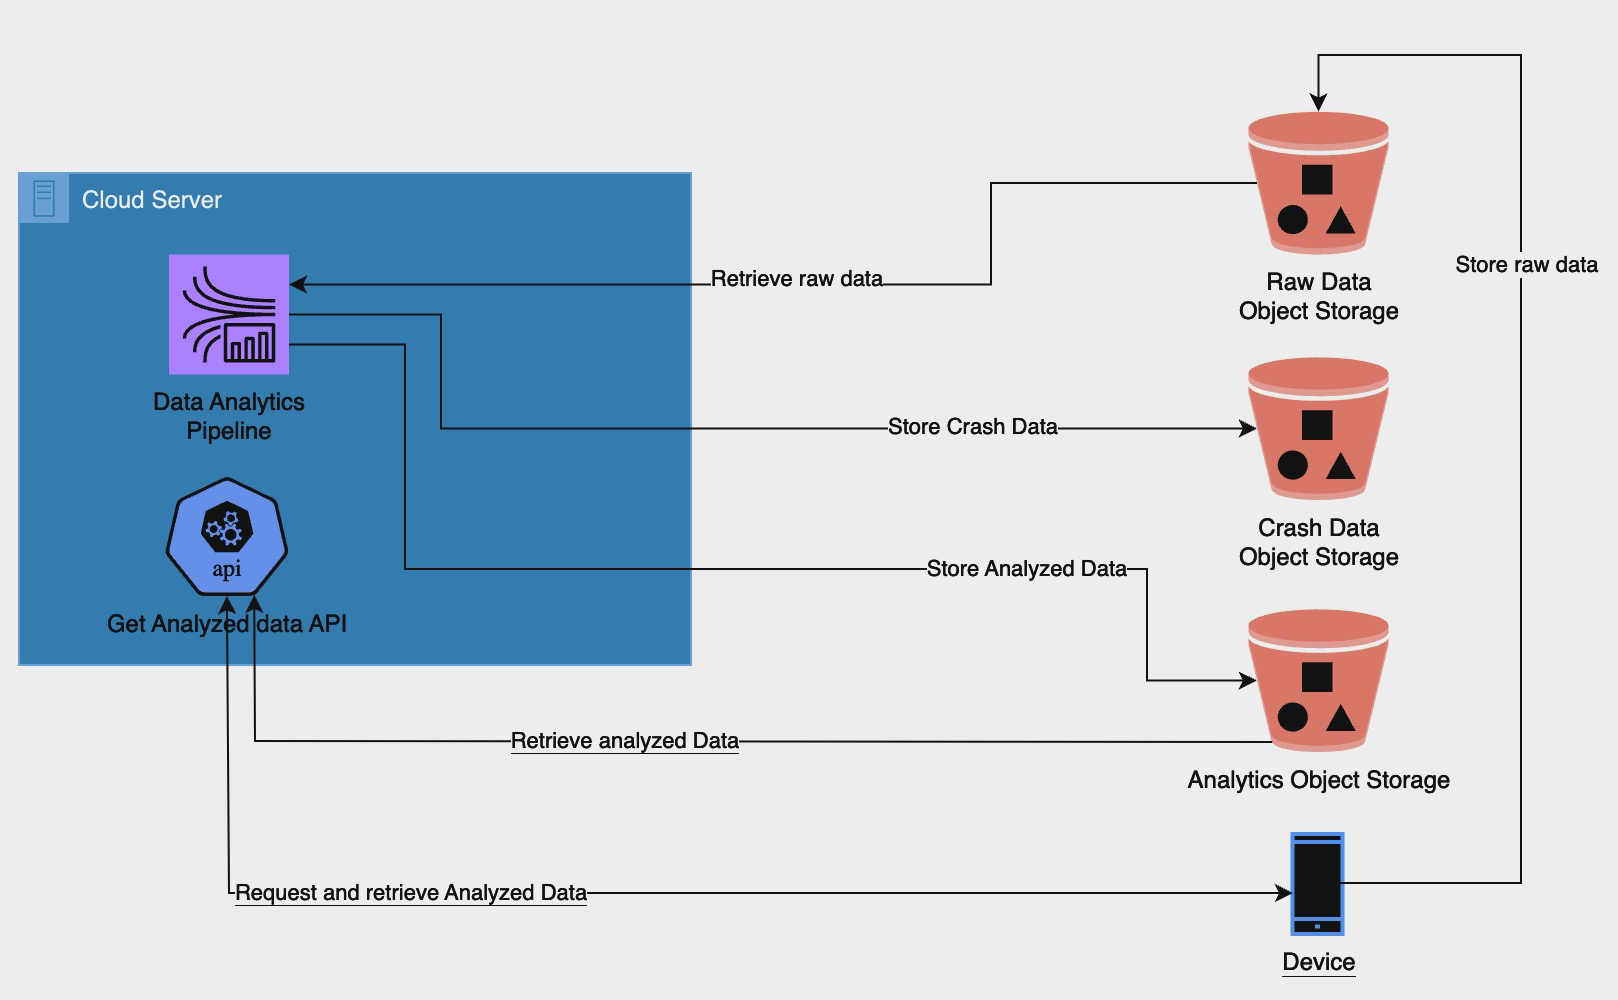
\includegraphics[width=1\textwidth]{preemptive_architecture.png}
    \caption{Architecture 1: Preemptive Analytics Processing}
\end{figure}

\subsubsection{Overview}
This architecture processes sensor data from biker suits as soon as it is received. The processed analytics are stored and readily available for users. This approach emphasizes real-time data processing to provide immediate insights and archive crash detection using Aruba's cloud services.

\subsubsection{Detailed Workflow}

\textbf{Data Ingestion}:  
Sensor data collected by the biker suit is uploaded to raw data object storage via app or dedicated hardware, ensuring a secure transfer and storage of data for subsequent processing.

\textbf{Trigger Analytics Pipeline}:  
A push event triggers a function or script on the Aruba Cloud Server to initiate the analytics pipeline. Alternatively, the pipeline can be triggered by an API (HTTP or WebSocket) call upon data upload.

\textbf{Data Processing}:  
The Aruba Cloud Server runs the data analytics pipeline, which involves several key stages:
\begin{itemize}
    \item \textbf{Data Preprocessing}: Cleaning and transforming raw data.
    \item \textbf{Analytics}: Applying algorithms to analyze the data.
    \item \textbf{Crash Detection}: Utilizing specific algorithms to detect crash events.
\end{itemize}

\textbf{Storage}:  
Processed analytics data is stored in a separate storage bucket within Aruba object storage. If a crash is detected, the raw data is duplicated in a crash-specific bucket. The original raw data is programmatically deleted to manage storage capacity efficiently.

\textbf{User Access}:  
Users are notified when analytics are available. The API Gateway provides an endpoint for users to request analytics data. The API retrieves the requested analytics data from the analytics bucket.

\textbf{Data Listing}:  
An API endpoint lists available analytics data based on metadata, facilitating easier management and retrieval for users.

\subsubsection{Components}
\begin{itemize}
    \item \textbf{Aruba Object Storage}: For raw, analytics, and crash data storage.
    \item \textbf{API or Event-Driven Services on Aruba Cloud Server}: To trigger the analytics pipeline.
    \item \textbf{Aruba Cloud Server Instances}: For running the analytics pipeline.
    \item \textbf{APIs}: For data retrieval and listing.
\end{itemize}

\subsubsection{Pros and Cons}

\textbf{Pros}:
\begin{itemize}
    \item Immediate availability of analytics data.
    \item Timely crash detection and data saving.
    \item Suitable for applications requiring real-time monitoring.
\end{itemize}

\textbf{Cons}:
\begin{itemize}
    \item High resource usage due to continuous processing.
    \item Potentially high operational costs.
    \item Scalability challenges with high data volume.
\end{itemize}

\subsection{Architecture 2: On-Demand Analytics Processing}

\begin{figure}[htbp]
    \centering
    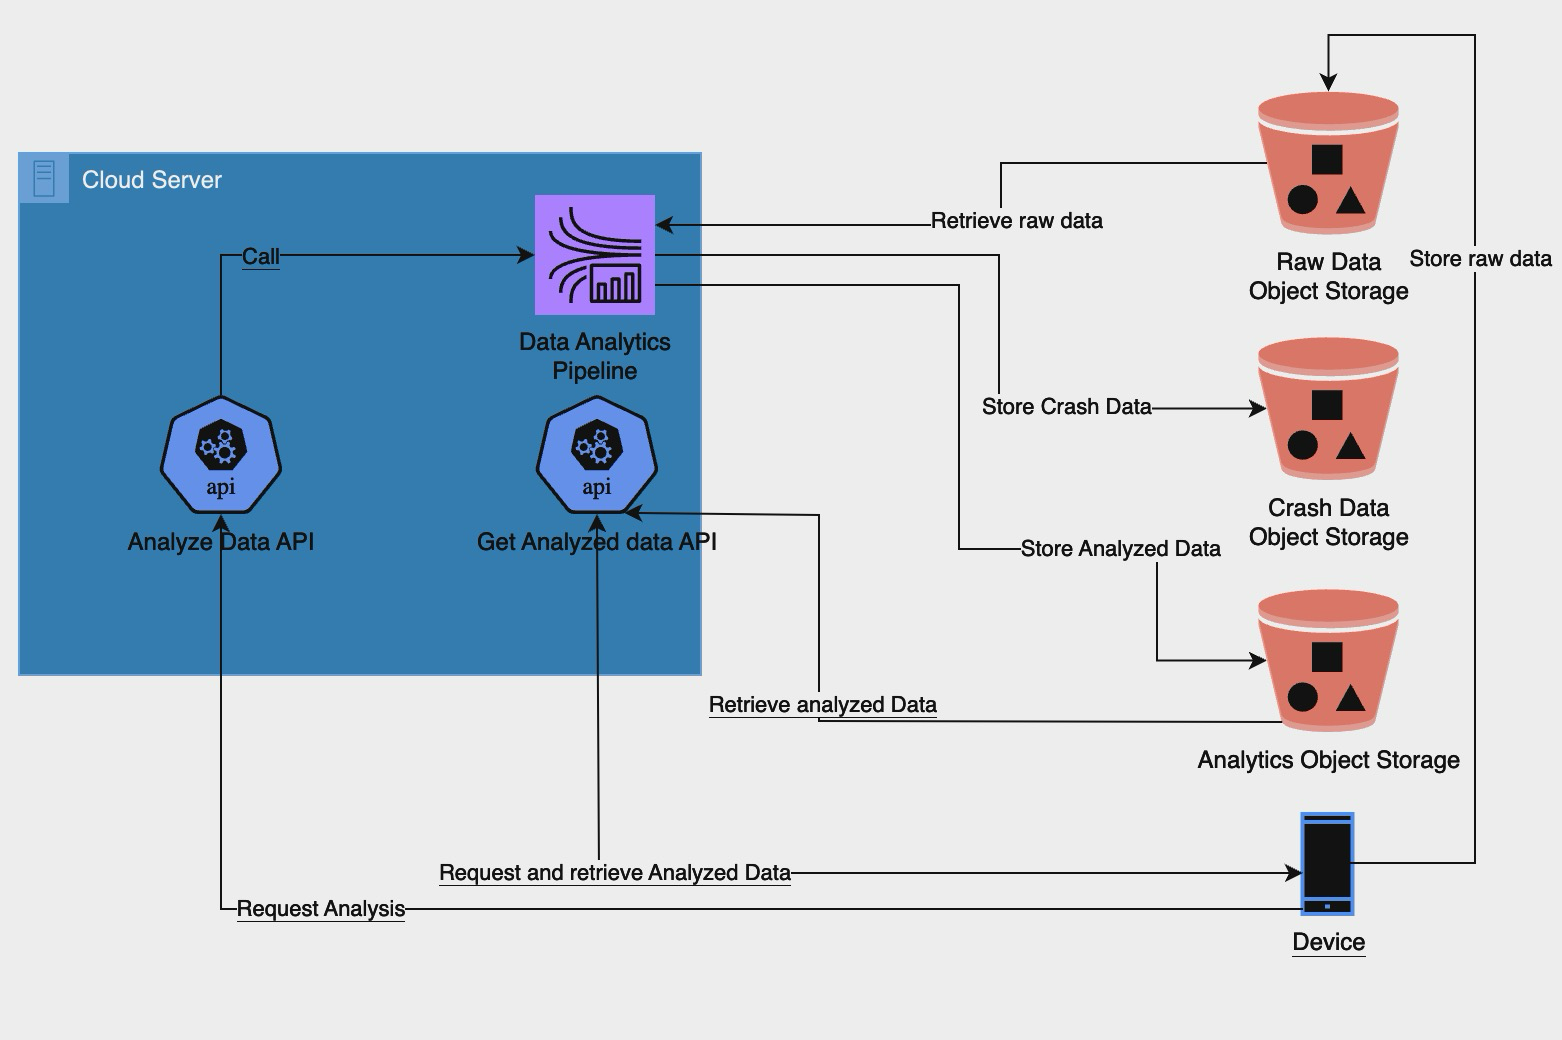
\includegraphics[width=1\textwidth]{on-demand_architecture.png}
    \caption{Architecture 2: On-Demand Analytics Processing}
\end{figure}

\subsubsection{Overview}
This architecture processes sensor data on demand. Users request analytics for specific dates, triggering the processing pipeline. This approach is resource-efficient, processing data only when necessary using Aruba's cloud services.

\subsubsection{Detailed Workflow}

\textbf{Data Ingestion}:  
The initial stage involves collecting sensor data from the biker suit. This data is uploaded to raw data object storage via mobile application or dedicated hardware, ensuring a secure transfer from the suit to a storage location where it can be accessed and processed.

\textbf{Data Listing}:  
After ingestion, the Listing API is utilized. This API endpoint lists all available raw data based on its metadata, facilitating easier management and retrieval for subsequent processing steps.

\textbf{Analytics Request}:  
The user requests data analytics through an API endpoint or a WebSocket at this stage. Upon receiving the request, a background job is triggered on the Aruba Cloud Server, initiating the analytics pipeline for processing the requested data.

\textbf{Data Processing}:  
Data processing involves several sub-stages on the Aruba Cloud Server:
\begin{itemize}
    \item \textbf{Data Preprocessing}: Raw data is cleaned and transformed to prepare it for analysis.
    \item \textbf{Analytics}: Algorithms are applied to analyze the data and extract meaningful insights.
    \item \textbf{Crash Detection}: Specialized algorithms detect crash events within the data.
\end{itemize}

\textbf{Storage}:  
After processing, the resulting analytics data is stored in a designated analytics bucket within the Aruba object storage. If a crash is detected, the raw data is duplicated in a crash-specific bucket. To efficiently manage storage capacity, the original raw data is programmatically deleted after processing.

\textbf{User Access}:  
In the final stage, the processed data is made available to the user. Users are notified via WebSocket if they made the analytics request through this method. The API Gateway provides an endpoint for users to request the analytics data, which is retrieved from the analytics bucket and delivered to the user.

\subsubsection{Components}
\begin{itemize}
    \item \textbf{Aruba Object Storage}: For raw, analytics, and crash data storage.
    \item \textbf{Job triggering API}: To handle on-demand processing.
    \item \textbf{Aruba Cloud Server Instances}: For running the analytics jobs.
    \item \textbf{APIs}: For data retrieval and listing.
\end{itemize}

\subsubsection{Pros and Cons}

\textbf{Pros}:
\begin{itemize}
    \item Resource-efficient with on-demand processing.
    \item Easier to scale due to reduced continuous load.
    \item Cost-effective due to lower operational costs.
\end{itemize}

\textbf{Cons}:
\begin{itemize}
    \item Delays in providing analytics data due to on-demand processing.
    \item Requires robust job scheduling and management.
\end{itemize}

\subsection{Comparative Summary}

\begin{longtable}{|p{3cm}|p{5cm}|p{5cm}|}
\hline
\textbf{Aspect} & \textbf{Architecture 1 (Preemptive)} & \textbf{Architecture 2 (On-Demand)} \\
\hline
\textbf{Data Processing} & Continuous & On-demand \\
\hline
\textbf{User Experience} & Immediate insights & High delays \\
\hline
\textbf{Resource Usage} & High & Optimized \\
\hline
\textbf{Scalability} & Challenging & Easier \\
\hline
\textbf{Cost Efficiency} & Potentially costly & More cost-effective \\
\hline
\textbf{Crash Detection} & Immediate & On-demand \\
\hline
\caption{Architecture Comparison}
\label{table:architecture_comparison}
\end{longtable}
Both Architecture 1 (Preemptive Analytics Processing) and Architecture 2 (On-Demand Analytics Processing) have distinct advantages and considerations. Architecture 1 was chosen primarily for its emphasis on real-time data processing and the immediate availability of analytics insights. This architecture ensures that sensor data from biker suits is processed as soon as it is received, enabling timely crash detection and data storage. The continuous processing nature of Architecture 1 supports applications requiring real-time monitoring, despite potential challenges in resource usage and scalability. Another important factor in selecting Architecture 1 is the client's focus on user experience and the need for immediate insights to enhance rider safety and performance.


\section{Implementation}
\label{sec:implementation}

In this section, we delve into the implementation of the chosen system architecture, detailing the various steps undertaken to bring the proposed solution to life. Architecture 1, the Preemptive Analytics Processing architecture, was selected due to its emphasis on real-time data processing and the immediate availability of analytics insights, aligning well with the client's focus on enhancing rider safety and performance. This section will outline the rationale behind choosing Architecture 1 and then walk through the implementation steps, ensuring each aspect of the system is comprehensively addressed.

\subsection{Rationale for Choosing Architecture 1}
Architecture 1 was chosen over Architecture 2 due to several key factors:
\begin{itemize}
    \item \textbf{Real-time Data Processing}: Architecture 1 supports the immediate processing of sensor data as soon as it is received, providing timely insights and crash detection, which are critical for enhancing rider safety and performance.
    \item \textbf{Immediate Availability of Analytics}: Users can access processed analytics data almost instantly, ensuring that the insights are available when needed without delays.
    \item \textbf{User Experience}: The client prioritized user experience, particularly for professional users and high-intensity private users who require quick feedback on their performance.
    \item \textbf{Crash Detection}: The ability to detect crashes immediately and store relevant data for further analysis was a significant requirement that Architecture 1 could efficiently handle.
\end{itemize}

Given these considerations, Architecture 1 was the optimal choice for the client's needs, providing the necessary real-time capabilities and user experience enhancements.

\subsection{Implementation Steps}
The implementation of Architecture 1 involved several crucial steps, each designed to ensure the system met the client's requirements for data handling, processing, and user interaction. It's worth mentioning that the first implementation has been treated as a PoC (Proof of Concept), in the description of the following steps will be mentioned which steps have been implemented in the PoC and which ones are yet to be developed.

\subsubsection{Data Ingestion}
The initial step in the implementation process was to establish a robust data ingestion mechanism. Sensor data collected by the biker suits needed to be securely uploaded to raw data object storage.

\textbf{Steps:}
\begin{enumerate}
    \item \textbf{Mobile Application Integration}: Develop or integrate a mobile application to facilitate data upload from the biker suit to the cloud. Ensure the app supports secure data transfer protocols.
    \item \textbf{Dedicated Hardware}: If applicable, implement dedicated hardware to manage data upload directly from the suit to the cloud, bypassing the need for a mobile app.
    \item \textbf{Secure Transfer}: Utilize secure transfer methods (e.g., HTTPS, SSL/TLS) to ensure data integrity and confidentiality during upload.
    \item \textbf{Object Storage Setup}: Configure Aruba Object Storage to receive and store raw sensor data securely.
\end{enumerate}

For the PoC, the Secure Transfer and Object Storage Setup steps have been implemented. To manage the file upload from the biker suit, a simple script was developed to simulate the data transfer process. The mobile application integration and dedicated hardware components will be considered in the next phase of development.



\subsubsection{Trigger Analytics Pipeline}
Upon successful data upload, an event or API call triggers the analytics processing pipeline on the Aruba Cloud Server.

\textbf{Steps:}
\begin{enumerate}
    \item \textbf{Event-Driven Services}: Implement event-driven services using cloud functions or serverless architecture to trigger the analytics pipeline upon data upload.
    \item \textbf{API Integration}: Develop APIs to allow manual or automated triggering of the analytics pipeline via HTTP or WebSocket calls.
\end{enumerate}

For the PoC, the trigger mechanism was simulated using an API call at the end of the data upload script. Whether to keep this approach or to implement an event-driven service will be decided based on the system's performance and client feedback as well as the cloud provider's capabilities.
\subsubsection{Data Processing}
The core of the implementation involves processing the uploaded sensor data through various stages, including preprocessing, analytics, and crash detection.

\textbf{Steps:}
\begin{enumerate}
    \item \textbf{Data Preprocessing}: Develop scripts or functions to clean and transform raw data, preparing it for analysis.
    \item \textbf{Analytics Algorithms}: Implement algorithms to analyze the preprocessed data, extracting insights related to rider performance.
    \item \textbf{Crash Detection Algorithms}: Develop specialized algorithms to detect crash events within the data, ensuring timely identification and response.
\end{enumerate}

The PoC implementation of the analytics pipeline was developed as a background subroutine triggered by the API call at the end of the data upload script. In this phase a simple set of metrics was calculated, e.g. Average speed, maximum acceleration, number of left and right turns, maximum deceleration, etc. The next steps will involve refining the preprocessing, analytics, and crash detection algorithms to provide more detailed and actionable insights.

\subsubsection{Storage of Processed Data}
Processed analytics data needs to be stored in a dedicated storage bucket, with special handling for crash data.

\textbf{Steps:}
\begin{enumerate}
    \item \textbf{Analytics Data Storage}: Configure a separate storage bucket within Aruba Object Storage for processed analytics data.
    \item \textbf{Crash Data Handling}: Implement mechanisms to duplicate raw data in a crash-specific bucket if a crash is detected. Ensure original raw data is programmatically deleted post-processing to manage storage capacity efficiently.
\end{enumerate}

For the PoC implementation, a separate storage bucket was set up to store the processed analytics data. The crash data handling mechanism will be developed in the next phase to ensure that crash events are detected and stored appropriately.
In both cases, the analytics and crash data are directly uploaded by the analytics pipeline described in the previous step.

\subsubsection{User Access and Notification}
Users must be notified when analytics are available and should have seamless access to retrieve their data.

\textbf{Steps:}
\begin{enumerate}
    \item \textbf{User Notification}: Implement push notifications or WebSocket notifications to inform users when their analytics data is ready.
    \item \textbf{API Gateway}: Set up an API Gateway to provide endpoints for users to request and retrieve analytics data.
    \item \textbf{Metadata Listing}: Develop API endpoints to list available analytics data based on metadata, facilitating easier data management and retrieval.
\end{enumerate}

For the PoC the API Gateway has been set up to provide an endpoint for users to request their analytics data. The metadata listing functionality has been implemented as an API endpoint to list available analytics data based on metadata. The user notification system will be developed in the next phase to ensure users are informed when their analytics data is ready for access.

\subsubsection{Data Retention and Management}
Ensure proper data retention policies are in place to manage storage efficiently while retaining essential metrics and crash data.

\textbf{Steps:}
\begin{enumerate}
    \item \textbf{Permanent Metrics Storage}: Store key metrics permanently, ensuring long-term availability for analysis and user access.
    \item \textbf{Temporary Raw Data Storage}: Implement policies to store raw data temporarily (2-4 weeks), unless a crash event is detected.
    \item \textbf{User Download Window}: Provide users with a time window to download and save their raw data before it is deleted.
\end{enumerate}

For the PoC, the permanent metrics storage has been implemented, ensuring that key metrics are stored securely for long-term access. The raw data cleaning has been developed as a batch process to manage storage capacity efficiently. The user download window functionality will be developed in the next phase to allow users to access and save their raw data before it is deleted.

\subsection{Technical Detail and Tools}
The implementation of the proposed solution involved the use of various tools and technologies to ensure the system's robustness, scalability, and efficiency. The following technical details provide an overview of the tools used in the implementation process:
\subsubsection{Cloud server}
Aruba cloud server instances were used to host the API Gateway, analytics pipeline, and other backend services. The cloud server provided a scalable and reliable environment for running the analytics pipeline and managing user requests.

\subsubsection{Aruba Object Storage}
Aruba Object Storage was used to store raw sensor data, processed analytics data, and crash data. It provides a secure and scalable storage solution for managing large volumes of data efficiently.
The storage is divided into three main buckets:
\begin{itemize}
    \item \textbf{Raw Data}: For storing the raw sensor data uploaded from the biker suits.
    \item \textbf{Analytics Data}: For storing the processed analytics data generated by the analytics pipeline.
    \item \textbf{Crash Data}: For storing the raw data in case a crash event is detected.
\end{itemize}

\subsubsection{API Gateway}
The API Gateway was used to provide endpoints for users to request and retrieve their analytics data. It acts as a central entry point for API requests, enabling seamless communication between users and the system.
The API Gateway provide a set of different APIs:
\begin{itemize}
    \item \textbf{Calculate Analytics}: An endpoint to trigger the analytics pipeline for a specific data set.
    \item \textbf{Retrieve Analytics}: An endpoint to retrieve the requested analytics data.
    \item \textbf{List Data}: An endpoint to list available data based on metadata, usable for RAW, Analytics and Crash data.
\end{itemize}

The API Gateway was first implemented using Python and FAST API, because of the simplicity and the speed of development.
Since performance issues were pretty evident even with a small number of concurrent users, the API Gateway was then reimplemented using Java and Spring Boot and deployed on Wildfly (Executed as a Linux service), which provided better performance and scalability. A detailed comparison between Java and Python for API development can be found in \ref{sec:java-vs-python}, while a description of how to start an application as a Linux service can be found in \ref{sec:cron-jobs}.
The implemented API Gateway already support TLS/SSL encryption and a basic authentication system, but it will be further improved in the next phase to support more advanced security features.

\subsubsection{Batch Processing}
Batch processing was mainly used to clean the raw data and manage storage capacity efficiently. The batch process runs periodically to clean up old raw data and ensure that storage space is optimized. Batch processing was implemented using Python scripts and scheduled to run at specific intervals, leveraging Linux cron jobs for automation. A more detailed description of cron jobs can be found in \ref{sec:cron-jobs}.

\section{Testing}
\label{sec:testing}
After the implementation of the system, a series of tests were conducted to ensure that the system met the client's requirements and performed as expected. The testing phase involved various types of tests, including unit tests, integration tests, and performance tests, to validate the system's functionality, reliability, and scalability.

\subsection{Unit Testing}
Unit tests were conducted to verify the functionality of individual components of the system, such as upload scripts, API endpoints and data cleaning processes. Even if this is not a best practice, unit tests were performed manually to ensure that each component worked as intended and produced the expected output. The unit tests were conducted in a controlled environment to isolate each component and identify any potential issues or bugs. In a future phase, a more comprehensive unit testing framework will be implemented to automate the testing process and ensure that all components are thoroughly tested.

\subsection{Integration Testing}
Integration tests were performed to validate the interactions between different components of the system, such as the API Gateway, analytics pipeline, and object storage. The integration tests focused on verifying that the components worked together seamlessly and communicated effectively to process and store data accurately. The integration tests were conducted in a test environment that replicated the production setup to ensure that the system would perform as expected in a real-world scenario.
These tests were performed manually, but in the next phase, an automated integration testing framework will be implemented to streamline the testing process and ensure that all components are integrated correctly.

\subsection{Performance Testing}
Performance tests were conducted to evaluate the system's scalability, reliability, and responsiveness under various load conditions. The tests measured the system's throughput, latency, and resource utilization to identify bottlenecks or performance issues. An automated stress test script simulated a high number of concurrent users accessing the system and uploading data. Initial performance issues were identified with the API Gateway developed in Python, leading to a reimplementation in Java and Spring Boot. The subsequent performance tests validated the improvements.
It's worth mentioning that these tests have been performed on a single server with a subset of users, in the next phase the system will be deployed on multiple servers to evaluate its performance in a distributed environment.
\newline
The results of the stress tests performed on the Python implementation of the API Gateway are not presented here, as they are not relevant to the final implementation. The results of the stress tests performed on the Java API Gateway are summarized in the following table:

\begin{table}[htbp]
\centering
\begin{tabular}{|c|c|c|c|}
\hline
\textbf{Number of Users} & \textbf{Calculate Analytics} & \textbf{Retrieve Analytics} & \textbf{List Data} \\
\hline 1 & 30 sec & 221 ms & 234 ms \\
\hline 10 & 85 sec (1 min 25 sec) & 252 ms & 228 ms \\
\hline 50 & 467 sec (7 min 47 sec) & 327 ms & 227 ms \\
\hline 250 & 2284 sec (38 min 4 sec) & 268 ms & 301 ms \\
\hline
\end{tabular}
\caption{Performance Metrics for Calculating, Retrieving, and Listing Analytics}
\label{table}
\end{table}

\subsubsection{Analysis of Results}
The performance metrics indicate how the system handles different numbers of concurrent users for three operations: Calculate Analytics, Retrieve Analytics, and List Data. Below is an analysis of the results:

\begin{itemize}
\item \textbf{Calculate Analytics}:
    \begin{itemize}
    \item With 1 user, the operation takes 30 seconds.
    \item As the number of users increases to 10, the time rises significantly to 85 seconds.
    \item For 50 users, the time increases drastically to 467 seconds.
    \item With 250 users, the operation takes 2284 seconds.
    \item The significant increase in time with more users suggests that the system experiences a performance bottleneck when calculating analytics under high load, the performance bottleneck is mainly due to the high number of data being transferred from the object storage to the analytics pipeline in the server.
    \item Even if the performance is not optimal, the 40 minutes required to calculate the analytics for 250 users is still acceptable for the client's requirements as the operation is not time-sensitive and would be performed while the users are charging their devices.
    \end{itemize}

\item \textbf{Retrieve Analytics}:
    \begin{itemize}
        \item The response time for retrieving analytics is relatively stable, ranging from 221 ms to 327 ms as the number of users increases from 1 to 250.
        \item The relatively minor variations in response time indicate that the system handles retrieving analytics efficiently, even under higher loads.
    \end{itemize}

\item \textbf{List Data}:
    \begin{itemize}
        \item The response time for listing data remains relatively consistent, ranging from 227 ms to 301 ms as the number of users increases from 1 to 250.
        \item This consistency indicates that the system efficiently handles the listing of data without significant performance degradation under load.
    \end{itemize}
\end{itemize}

\subsubsection{Conclusion}
The performance tests highlight that while the system handles retrieving and listing data efficiently under increasing loads, calculating analytics exhibits significant performance degradation as the number of users increases. Since the bottleneck is mainly due to the high number of data being transferred from the object storage to the analytics pipeline in the server, the next phase will focus on optimizing the data transfer process to improve the system's performance. The quickest solution would be to use more, less powerful servers to distribute the load. The system could also be optimized by saving raw data directly in the server, but this would require a significant amount of storage space and would not be scalable in the long run as well as the higher cost of the storage. The best solution would be to deploy the application in a containerized environment, using Kubernetes to manage the containers and distribute the load among different servers. This would allow the system to scale horizontally, adding more servers as needed, and would also provide a more efficient way to manage the data transfer process.
